\item \textbf{{[}PJC/PRELIM/9597/2014/P1/Q3{]} }

Implement a linked list to store names of runners and their best running
times in seconds, in ascending order of running time. The runner with
the fastest timing is stored at the first node while the runner with
the slowest timing is stored at the last node. A linked list of free
nodes is also implemented with a maximum size of 20 nodes. 

The program will use a user-defined type \texttt{Node} for each node
defined as follows: 
\begin{center}
\begin{tabular}{|l|l|l|}
\hline 
\texttt{\textbf{\hspace{0.01\columnwidth}}}\textbf{Identifier} & \texttt{\textbf{\hspace{0.01\columnwidth}}}\textbf{Data Type} & \texttt{\textbf{\hspace{0.05\columnwidth}}}\textbf{Description}\tabularnewline
\hline 
\texttt{Name} & \texttt{STRING} & The name of the runner\tabularnewline
\hline 
\texttt{Time} & \texttt{FLOAT} & The best running time of the runner\tabularnewline
\hline 
\texttt{Next} & \texttt{POINTER} & The pointer to the next node \tabularnewline
\hline 
\end{tabular}
\par\end{center}

The program will also use another user-defined type \texttt{LinkedList}
for each linked list. It contains a \texttt{first} pointer that points
to the first node of the linked list and makes use of \texttt{Node}
for its nodes. 

The user-defined type LinkedList contains methods as follows: 
\begin{center}
\begin{tabular}{|l|l|}
\hline 
\texttt{\textbf{\hspace{0.01\columnwidth}}}\textbf{Method} & \texttt{\textbf{\hspace{0.05\columnwidth}}}\textbf{Description}\tabularnewline
\hline 
\texttt{Display } & To display the contents of the linked list in order \tabularnewline
\hline 
\texttt{AddFirst } & To add a new node as first node of linked list\tabularnewline
\hline 
\texttt{RemoveFirst } & To remove first node of linked list\tabularnewline
\hline 
\texttt{AddLast} & To add a new node as last node of linked list \tabularnewline
\hline 
\texttt{RemoveLast} & To remove last node of linked list\tabularnewline
\hline 
\texttt{Empty} & To return Boolean True if linked list is empty\tabularnewline
\hline 
\end{tabular}
\par\end{center}

The diagram shows two linked lists -- \texttt{RaceList} and \texttt{FreeList}.

\texttt{RaceList} contains a dataset of four nodes. Each node contains
a \emph{name}, a \emph{running time}, and a \emph{pointer} to the
next node. 

\texttt{FreeList} is a list of free nodes available for \texttt{RaceList}
to store data, where the maximum number of nodes is 20.
\begin{center}
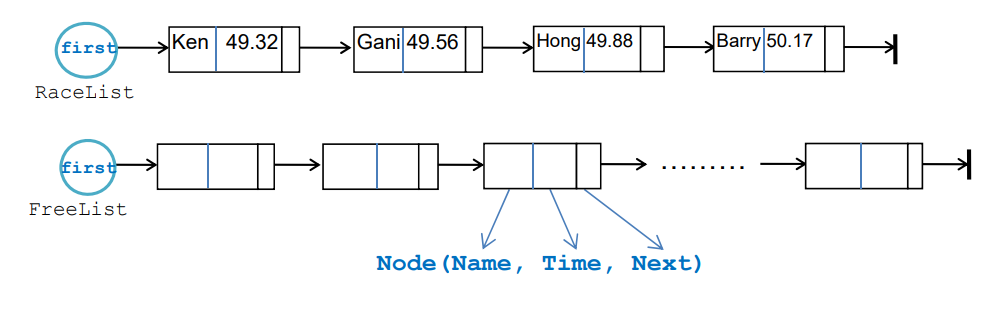
\includegraphics[width=0.65\paperwidth]{C:/Users/Admin/Desktop/Github/question_bank/LyX/static/img/9597-PJC-2014-P1-Q3}
\par\end{center}

\subsection*{Task 3.1 }

Write program code to create \texttt{Node} and \texttt{LinkedList},
and initialise an empty linked \texttt{RaceList}, and \texttt{FreeList}
of \textbf{20} nodes. Ensure all identifiers and methods specified
above are created. 

\subsection*{Evidence 8: }

Your program code for task 3.1. \hfill{}{[}17{]}

\subsection*{Evidence 9: }

Screenshot of running method to display \texttt{RaceList} and \texttt{FreeList}
on screen. \hfill{}{[}1{]}

\subsection*{Task 3.2 }

Write code to implement a method \texttt{AddInOrder} that will add
a new node with data into \texttt{RaceList} in ascending order of
running time. Node added to \texttt{RaceList} should be taken from
\texttt{FreeList}. 

\subsection*{Evidence 10: }

Your program code for task 3.2. \hfill{}{[}11{]}

\subsection*{Task 3.3 }

Test your program using the following data items input in the order
shown and run method to display \texttt{RaceList} and \texttt{FreeList}
on screen. 
\noindent \begin{center}
\begin{tabular}{|c|c|c|}
\hline 
\textbf{Order of input } & \textbf{Name} & \textbf{Running Time}\tabularnewline
\hline 
\hline 
1 & Barry & 50.17\tabularnewline
\hline 
2 & Gani  & 49.56\tabularnewline
\hline 
3 & Hong & 49.88\tabularnewline
\hline 
4 & Ken & 49.32 \tabularnewline
\hline 
\end{tabular} 
\par\end{center}

\subsection*{Evidence 11: }

Provide screenshot for task 3.3. \hfill{} {[}2{]}

\subsection*{Task 3.4 }

Write code to implement a method \texttt{RemoveNode} that will remove
the node that contains data specified by user to be removed from \texttt{RaceList}.
Node removed from \texttt{RaceList} should be returned to \texttt{FreeList}. 

\subsection*{Evidence 12: }

Your program code for task 3.4. \hfill{}{[}8{]}

\subsection*{Task 3.5 }

Test your program by removing \texttt{Gani} from \texttt{RaceList}
and run method to display \texttt{RaceL}ist and \texttt{FreeList}
on screen. 

\subsection*{Evidence 13: }

Provide screenshot for task 3.5. \hfill{} {[}1{]}